\documentclass{beamer}
\usetheme{default}
\setbeamertemplate{navigation symbols}{}
%	
\usepackage{subfig}
\usepackage{epstopdf}
\usepackage{amsmath, amsthm, amssymb}
\usepackage{float}
\usepackage{rotating}
\usepackage{graphicx}
\usepackage{longtable}
\usepackage{xcolor}
\usepackage{bm}
\usepackage{tikz}
\usetikzlibrary{shapes}
\tikzset{My Arrow Style/.style={single arrow, fill=red!50, anchor=base, align=center,text width=.5cm,rotate =270}}
\newcommand{\MyArrow}[2][]{\tikz[baseline] \node [My Arrow Style,#1] {#2};}
\tikzset{My 2Arrow Style/.style={single arrow, fill=red!50, anchor=base, align=center,text width=.5cm,rotate =90}}
\newcommand{\MyArrowUp}[2][]{\tikz[baseline] \node [My 2Arrow Style,#1] {#2};}
\newcommand{\EE}{\mathbb E}
\newcommand{\var}{\mathrm{var}}
\newcommand{\cov}{\mathrm{cov}}
\newtheorem{acknowledgement}[theorem]{Acknowledgement}
\newtheorem{algorithm}[theorem]{Algorithm}
\newtheorem{assumption}{Assumption}
\newtheorem{axiom}{Axiom}
\newtheorem{case}[theorem]{Case}
\newtheorem{claim}[theorem]{Claim}
\newtheorem{conclusion}[theorem]{Conclusion}
\newtheorem{condition}[theorem]{Condition}
\newtheorem{conjecture}{Conjecture}
\newtheorem{criterion}[theorem]{Criterion}
\newtheorem{proposition}{Proposition}
\newtheorem{summary}[theorem]{Summary}
\newtheorem{exercise}{Exercise}
\newtheorem{notation}{Notation}
\newtheorem{remark}{Remark}
%\graphicspath{{graphs//}}

\title {Taxes, Debts,  and Redistribution}
\author{Anmol Bhandari, David Evans, Mikhail Golosov, Thomas J. Sargent}

\date{September 2013}
% \today will show current date.
% Alternatively, you can specify a date.
%
\begin{document}
%
\begin{frame}
\titlepage

\end{frame}


\begin{frame}
\frametitle{3 Questions}

\begin{enumerate}
 \item How costly are government debts?
 \vspace{2mm} 
 \item How do concerns for redistribution affect tax smoothing motives?
\vspace{2mm} 
 \item Quantify how should tax, transfer and debt policies respond to aggregate shocks that change inequality?
\end{enumerate}

\end{frame}


\begin{frame}
\frametitle{Point of Departure: Representative agent models}
\textbf{Debt levels:}
\begin{itemize}
\item Higher levels of debt are generally ``more'' distortionary. 
\end{itemize}
\textbf{Tax smoothing:}
\begin{itemize}
 \item LS: With complete markets tax rates should be smooth.  
 \vspace{2mm} 
 \item Werning: Extends the LS insights to heterogeneous agents by establishing an aggregation result.
 \vspace{2mm} 
 \item AMSS: With a risk free bond, tax rates are eventually smooth and all aggregate shocks are financed using transfers.
\end{itemize}



\end{frame}

\begin{frame}
\frametitle{Implicit and explicit redistribution}
\begin{itemize}
\item Representative agent models implicitly model redistribution as a non-negativity constraint on lump sum transfers. 

\vspace{2mm} 
 \item Hardwires a discontinuity in the costs of fluctuating transfers around zero.
 \begin{enumerate}
  
 \item The Ramsey planner either uses state-contingent securities to hedge aggregate shocks. 
 
 \begin{center}or \end{center}
 
 \item Accumulates a war chest of assets big enough to finance expenditures using returns on assets plus only positive transfers.
 
 \end{enumerate}

 
\end{itemize}

\vspace{2mm} 
\emph{\color{red}We begin with explicit redistribution motives  and let the government set transfers optimally. }

%   \item Representative agent models impose restrictions on transfers
%   \begin{itemize}
%  \item These are motivated only implicitly by concerns about  redistribution:  poor people can't afford lump sum taxes
%   \item These constraints \emph{almost} always bind (e.g.,  Lucas Stokey, AMSS) and drive long run debt dynamics
%   \end{itemize}
% \item We begin with explicit redistribution motives  and let the government set transfers optimally
%  \end{itemize}
% 
%  \vspace{4mm}
%  \color{red}\emph{Prescriptions for optimal tax-transfers differ substantially with explicitly modeled redistribution concerns}
%  \end{frame}
% 
\end{frame}



\begin{frame}
\frametitle{Key ingredients}


\begin{itemize}
\vspace{3mm}
 \item \textbf{Heterogeneity:} Agents are heterogeneous in productivities and assets 

 \item \textbf{Instruments:} A tax system that is affine in labor income
 \vspace{3mm}
 \item \textbf{Markets:} All agents trade a \emph{single} security whose payoffs can depend on aggregate shocks
\end{itemize}


\end{frame}

\begin{frame}
 \frametitle{Answers to the 3 questions}
 
\begin{enumerate}
\item \textbf{Invariance of  debt level:} 

Absent borrowing constraints, Ricardian equivalence holds. Borrowing constraints weakly increase welfare

\item \textbf{Invariant distribution of tax rates:} 

\begin{itemize}
	\item Has wide support
       \item The mean and variance of tax rates are driven by market incompleteness. The ``covariances'' that matter are 
       \begin{itemize}
        \item [+]  Between returns on the asset and aggregate shocks (Public sector)
        \item [+]  Between consumption and (	
        pre-tax) earnings (Private sector)
       \end{itemize}
\end{itemize}



\item \textbf{Business cycle dynamics:} (Preliminary) 
With countercyclical payoffs, tax rate and transfers increases with aggregate TFP.
\end{enumerate}



\end{frame}



\begin{frame}
 \frametitle{Environment}
 \begin{itemize}
 \item \textbf{Uncertainty}: Markov aggregate shocks $s_t$
  \item \textbf{Demography}: Continuum of infinitely lived agents plus a benevolent planner
  \item \textbf{Technology}: Output $\int \theta_{i,t} l_{i,t}di$ is linear in labor supplies.
  \item \textbf{Preferences }(Households)
  \begin{equation*}
\mathbb{E}_{0}\sum_{t=0}^{\infty } \beta^t U^{i}\left(
c_{i,t},l_{i,t}\right)  \label{utility lifetime}
\end{equation*}%
\item \textbf{Preferences} (Planner): Given Pareto weights $\{\omega_i\}$
\begin{equation*}
\mathbb{E}_{0}\int \omega_i\sum_{t=0}^{\infty }\beta^t U_{t}^{i}\left( c_{i,t},l_{i,t}\right)di  \label{govmt objective}
\end{equation*}
  \item \textbf{Asset markets}: A ``risky'' bond with payoffs $P_t=\mathbb{P}(s_t|s_{t-1})$
  \end{itemize}

\end{frame}



\begin{frame}
 \frametitle{Environment, II}
 \begin{itemize}
  \item \textbf{Affine Taxes}: Agent $i$'s tax bill
\[- T_t + \tau_t \theta_{i,t}l_{i,t}\]

\item[]
  \item \textbf{Budget constraints} Let $R_{t-1,t}=\frac{P_t}{q_{t-1}}$
  \begin{itemize}
   \item Agent $i$: $ c_{i,t}+b_{i,t}=\left( 1-\tau _{t}\right) \theta _{i,t}l_{i,t}+R_{t-1,t}b_{i,t-1}+T_{t}$
\item Government: $g_{t}+B_{t}+T_t=\tau _{t}\int \theta_{i,t}l_{i,t}di+R_{t-1,t}B_{t-1}$
  \end{itemize}

\item[]
  \item \textbf{Market Clearing}
  \begin{itemize}
   \item Goods: $\int c_{i,t}di+g_t =\int \theta _{i,t} l_{i,t}di$

   \item Assets: $\int b_{i,t}di +B_{t}=0$

  \end{itemize}
  \item[]

\item \textbf{Initial conditions}: Distribution of assets, productivities  $(\Psi_0(b_{i,-1}, \theta_{i,-1
}),B_{-1},s_{-1})$
\end{itemize}
\end{frame}



\begin{frame}
 \frametitle{Ramsey Problem}
\label{ramsey-problem}
\begin{definition}
\textbf{Allocation, price system, government policy}: Standard

\end{definition}

\begin{definition}
\textbf{Competitive equilibrium}: Given $\left( \Psi_0(b_{i,-1},\theta_{i,-1})
_{i},B_{-1},s_{-1}\right) $ and $\left\{ \tau _{t},T_{t}\right\} _{t=0}^{\infty }$
all allocations are chosen optimally, markets clear 
\end{definition}

\begin{definition}
\textbf{Optimal competitive equilibrium}: A welfare-maximizing competitive
equilibrium for a given $\left( \Psi_0(b_{i,-1},\theta_{i,-1}),B_{-1},s_{-1}\right) $
\end{definition}
\hyperlink{extra-slides}{\beamerbutton{Recursive formulation}}
 \end{frame}




 \begin{frame}
  \frametitle{Ricardian Equivalence}
  \begin{itemize}
   \item \textbf{Result}: A large set of transfers and asset profiles support the same competitive allocation
   
   \emph{Taking away a unit of all agents' assets and increasing transfers by a unit leaves budget sets unchanged}
   
   \vspace{2mm}
   
   \item \textbf{Implication:} Ceteris paribus, an economy with higher level of initial government debt  but same relative holdings has the same welfare
   
   \vspace{2mm}
   
   \item \textbf{Corollary:} Exogenous borrowing constraints of the form $b_{it}>\underline{b}_i$ are not restrictive
\vspace{2mm}
   
   
 \emph {If some borrowing constraints bind, the planner can change transfers to  slacken   \emph{all}  of them}
  \end{itemize}
  \color{red}\emph{Thus, Ricardian equivalence holds with distortionary taxes and ad hoc borrowing limits}

  
  
\end{frame}



\begin{frame}
 \frametitle{Active channels}
  \begin{enumerate}
\item Varying labor taxes imposes dead weight losses.


\item Effects of taxes on redistribution depends on cross sectional heterogeneity of consumption and earnings.

\item Fluctuating transfers is costly because of concerns for redistribution. 

\item The benefits of fluctuating transfers depend of limits to fiscal hedging.

\end{enumerate}

 \end{frame}


\begin{frame}
 \frametitle{Simple Example: 2 Agent QL economy}
 Consider a ``seemingly'' AMSS economy
 \begin{enumerate}
  \item Two classes of agent with constant productivities $\theta_1>0,\theta_2=0$
  \item Preferences given by $U(c,l)=c-\frac{l^{1+\gamma}}{1+\gamma}$
  \item Pareto weights $\{\omega,1-\omega\}$
  \item Only i.i.d aggregate shocks to $g(s)$
 \end{enumerate}
 
  
  In this example, 
  \begin{itemize}
   
   \item Costs of transfers will come from Pareto weights
   \item Hedging motive will be controlled using payoffs $P(s)$
  \end{itemize}


\end{frame}


\begin{frame}
 \frametitle{Case 1: Risk free bond}
 Normalize the assets of the unproductive agent to zero and let $b_t$ denote the debt issued by the government.
\begin{theorem}
Let $\omega>\bar{\omega}$ and  suppose $P(s)=1$, $\lim_t \tau_t=-\infty$, $\lim_t b_t=-\infty$     a.s
\end{theorem}

\vspace{3mm}

\begin{corollary} Suppose we augment our problem with a constraint $b_{t}\geq \underline{b}.$ Then with risk-free debt there is an invariant distribution $\psi .$ Morever, for any $\hat{b}\in \left( \underline{b},\bar{b}_n\right) ,$ $\psi \left( \left[ \underline{b},\hat{b}%
\right] \right) >0$ and $\psi \left( \left[ \hat{b},\bar{b}_n\right] \right)
>0.$. 
\end{corollary}


\vspace{3mm}
\emph{\color{red}The invariant distribution of taxes is wide as fluctuations in transfers are costly}

\end{frame}



\begin{frame}
 \frametitle{Case 2: Perfect hedging}
\begin{theorem}
Let $\omega>\bar{\omega}$ and suppose $\overline b < \overline b_n$ and payoffs satisfy
\[P(s) = 1- \frac{\beta}{\overline b}(g(s) - \mathbb{E} g)\] 
			 then for all $b_{-1}$, $b_t\rightarrow \overline b $ a.s 
\end{theorem}


\begin{corollary} The invariant distribution of $b$ (and also tax rates) is degenerate with $\bar{b}=-\beta\frac{\var[g(s)]}{\cov[P(s),g(s)]}$ 
\end{corollary}

\vspace{3mm}

\emph{\color{red} The limiting allocation corresponds to a complete market Ramsey problem}
\end{frame}


\begin{frame}
 \frametitle{Case 3: Imperfect hedging}

\textbf{Decompose payoffs} \[P(s)=\hat{P}(s)+\bar{P}(s)\] 

where	$\overline{P}(s) = 1- \frac{\beta}{\overline b}( g(s) - \mathbb{E} g)$ and  $\hat{P}(s)$ is orthogonal to $g(s)$. 

	

\begin{theorem}
For $\omega>\bar{\omega}$, the ergodic distribution of debt of the policy rules linearized around $(\overline b, \overline{P}(s))$ will have mean $\overline b$ and and coefficient of variation
	%
	\[
			\frac{\sigma_b} {\overline b} \leq 	\sqrt \frac{\var(\hat P)}  {\var(\bar{P})}
	\]

	The speed of convergence to the ergodic distribution given by
	\[
		\frac{\EE_{t-1}(b_t-\overline b)}{(b_{t-1} - \overline b)} = \frac1{1+|\cov(P(s),g(s))|}
	\]


\end{theorem}




\end{frame}






\begin{frame}
 \frametitle{More generally}
 
 \begin{enumerate}
  
 \item \textbf{Risk aversion}
 
 \begin{itemize}
  \item Endogenous component to covariance between payoffs and expenditure needs.
  
  \item Costs of transfers come from spreads in marginal utilities.
  
  
  \end{itemize}
  \vspace{3mm}
 \item \textbf{Idiosyncratic risk}
 \begin{itemize}
\item Joint distribution of consumption and pre-tax earnings drives the mean level of taxes
\item The spread of taxes is mainly a determined by public sector's fiscal hedging abilities

 \end{itemize}

\end{enumerate}

 \end{frame}
 
\begin{frame}
 \frametitle{Numerical example}
 
 
\textbf{Features:} 
\begin{itemize}
\item Continuum of agents
 
 \item Pre tax wage earnings with transitory and persistent component
 \item IID aggregate TFP shocks
 
 \end{itemize}
 
\textbf{Calibration:} 
 \begin{itemize}
 \item For now innovation to aggregate and idiosyncratic wages are orthogonal
 \item  Initial distribution of wages and earnings calibrated  to broadly match Díaz-Giménez et al
 
\end{itemize}
 
 \vspace{3mm}

 \color{red}{Study responses to aggregate shocks}

 
 \end{frame}

 
 \begin{frame}
  \frametitle{Findings}
  \begin{enumerate}

\item As before tax rates can drift in the long run.
\vspace{3mm}
\item In the short run what matters is how needs for redistribution change over business cycle.
\begin{itemize}

\item The heterogeneity in wealth effect drives how aggregate shocks affect the distribution of labor earnings
\item The cylicality of interest rate affect needs and costs of increasing transfers

\end{itemize}

\end{enumerate}


  \end{frame}

\begin{frame}
\frametitle{Bond Economy}
\begin{figure}[htp]
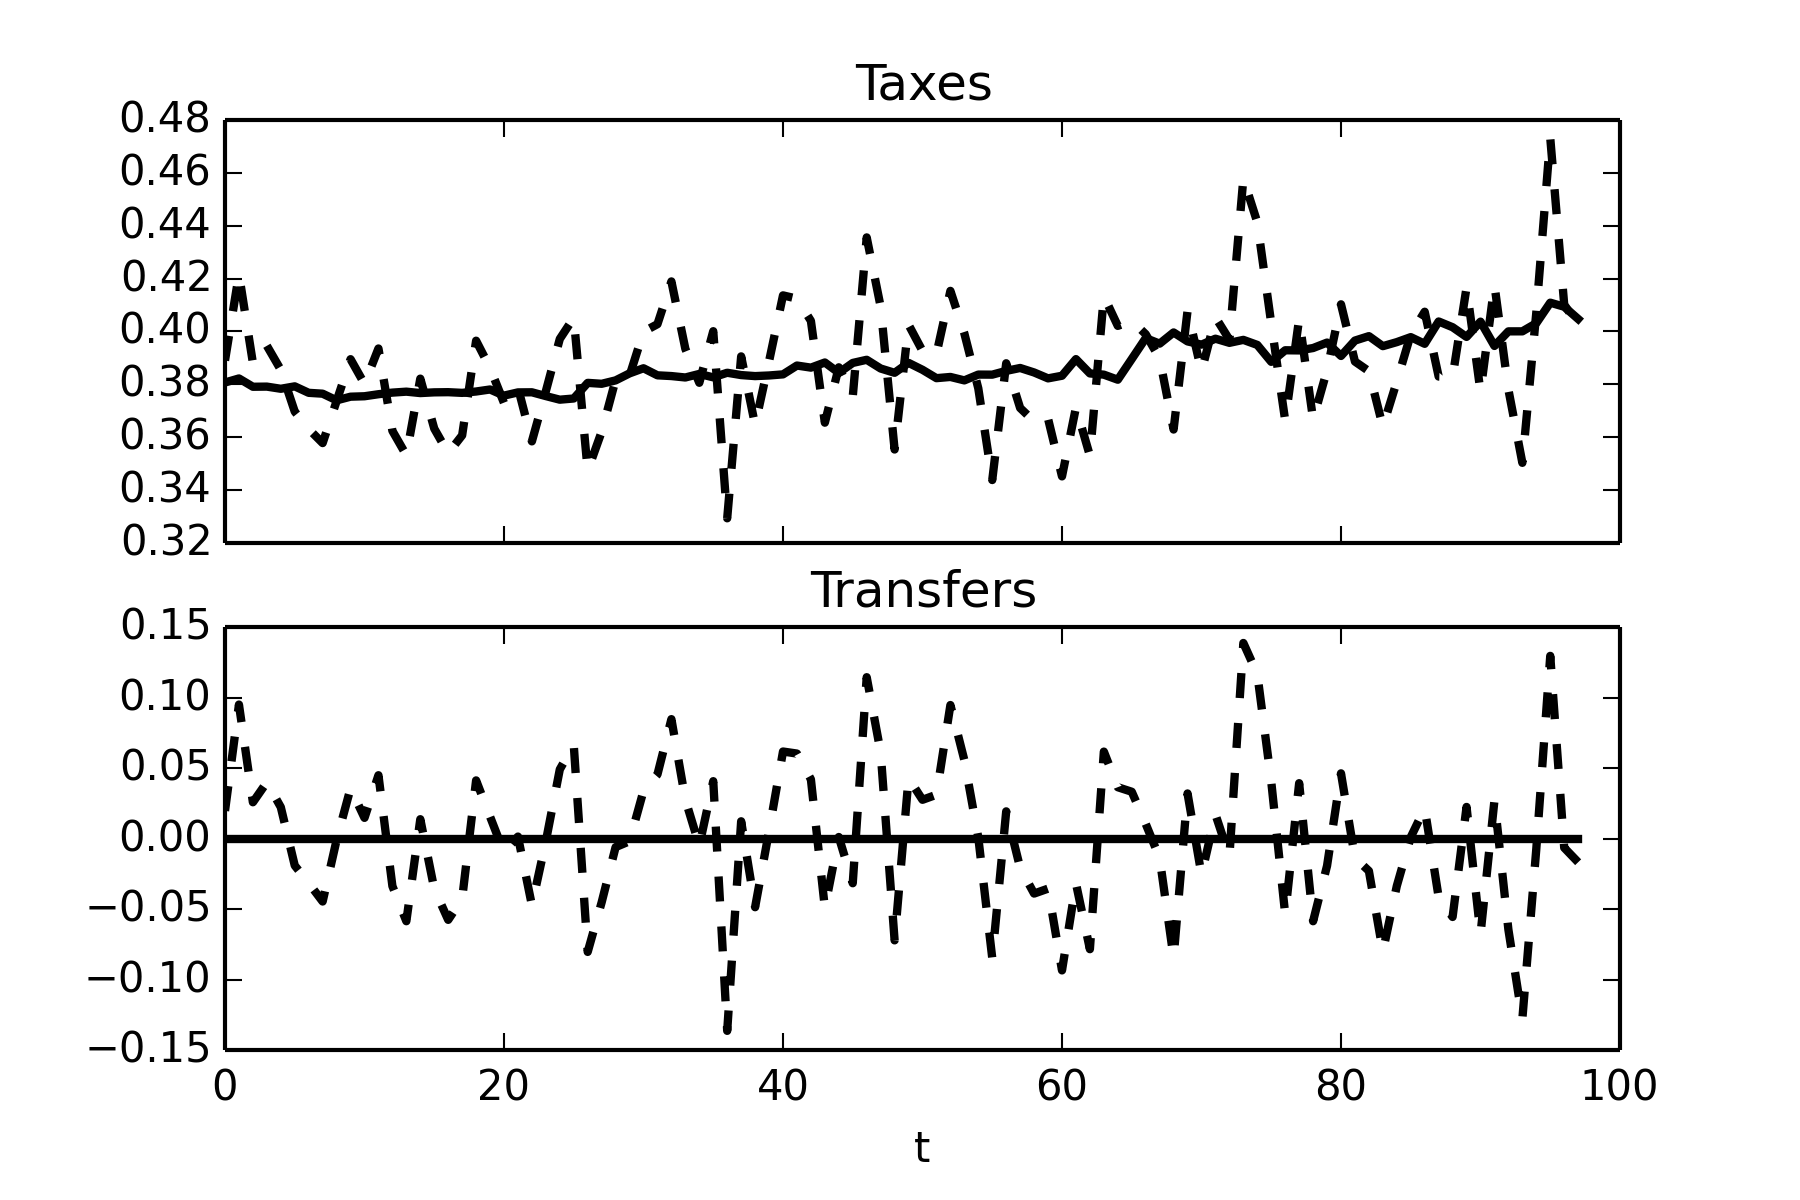
\includegraphics[width=\textwidth]{policy_long_sample_plot_data_bond_economy.png}
\caption{\tiny{This plots a simulation for taxes and transfers for 100 periods. The dotted (bold) line is the economy with (without) i.i.d aggregate shocks}}
\label{fig:}
\end{figure} 
\end{frame}
 
\begin{frame}
 \frametitle{Bond Economy}
\begin{figure}[htp]
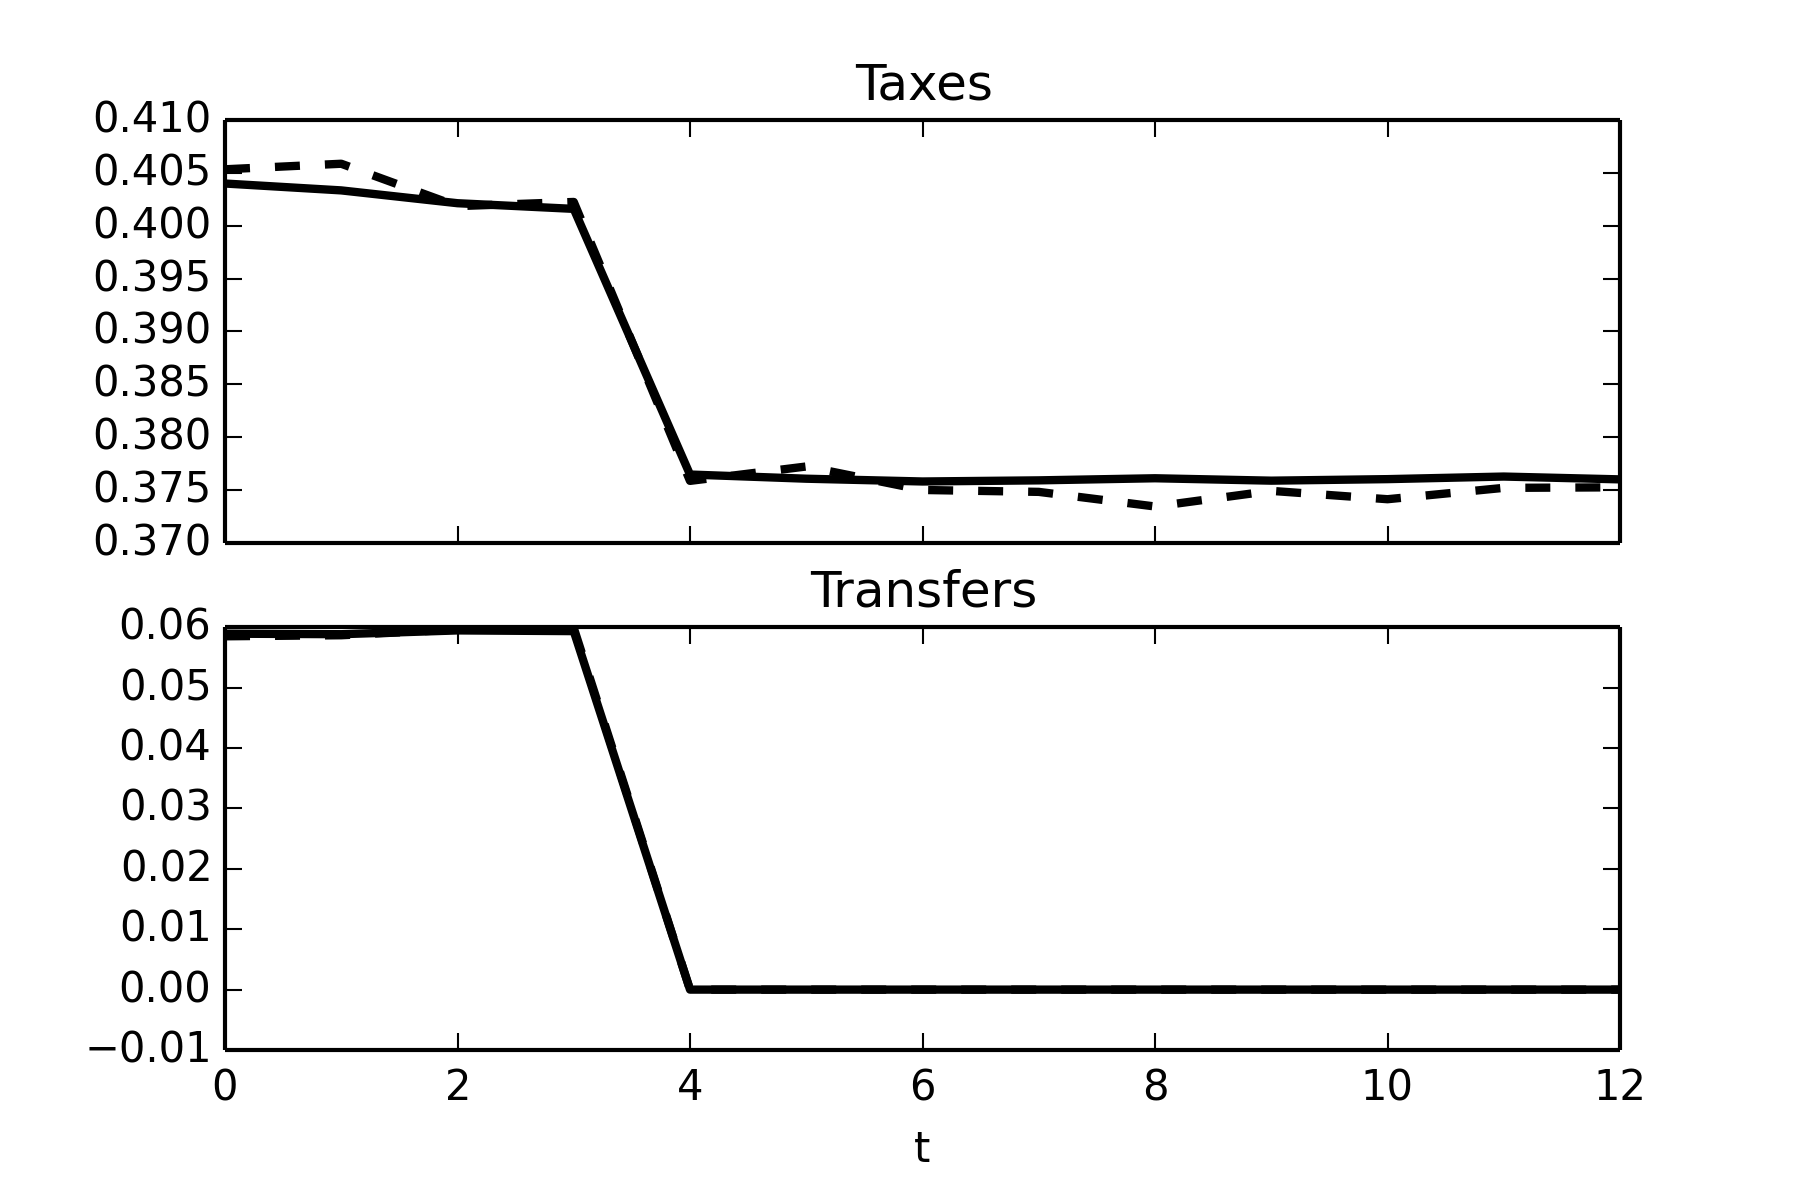
\includegraphics[width=\textwidth]{policy_irf_high_plot_data_bond_economy.png}
\caption{\tiny{This plots a ``impulse response'' (5 period of high aggregate TFP followed by no aggregate shocks) for taxes, transfers. The dotted (bold) line is the economy with (without) idiosyncratic risk}}
\label{fig:}
\end{figure}


 \end{frame}
 
 
\begin{frame}
 \frametitle{Changes in inequality: Bond Economy}
\begin{figure}[htp]
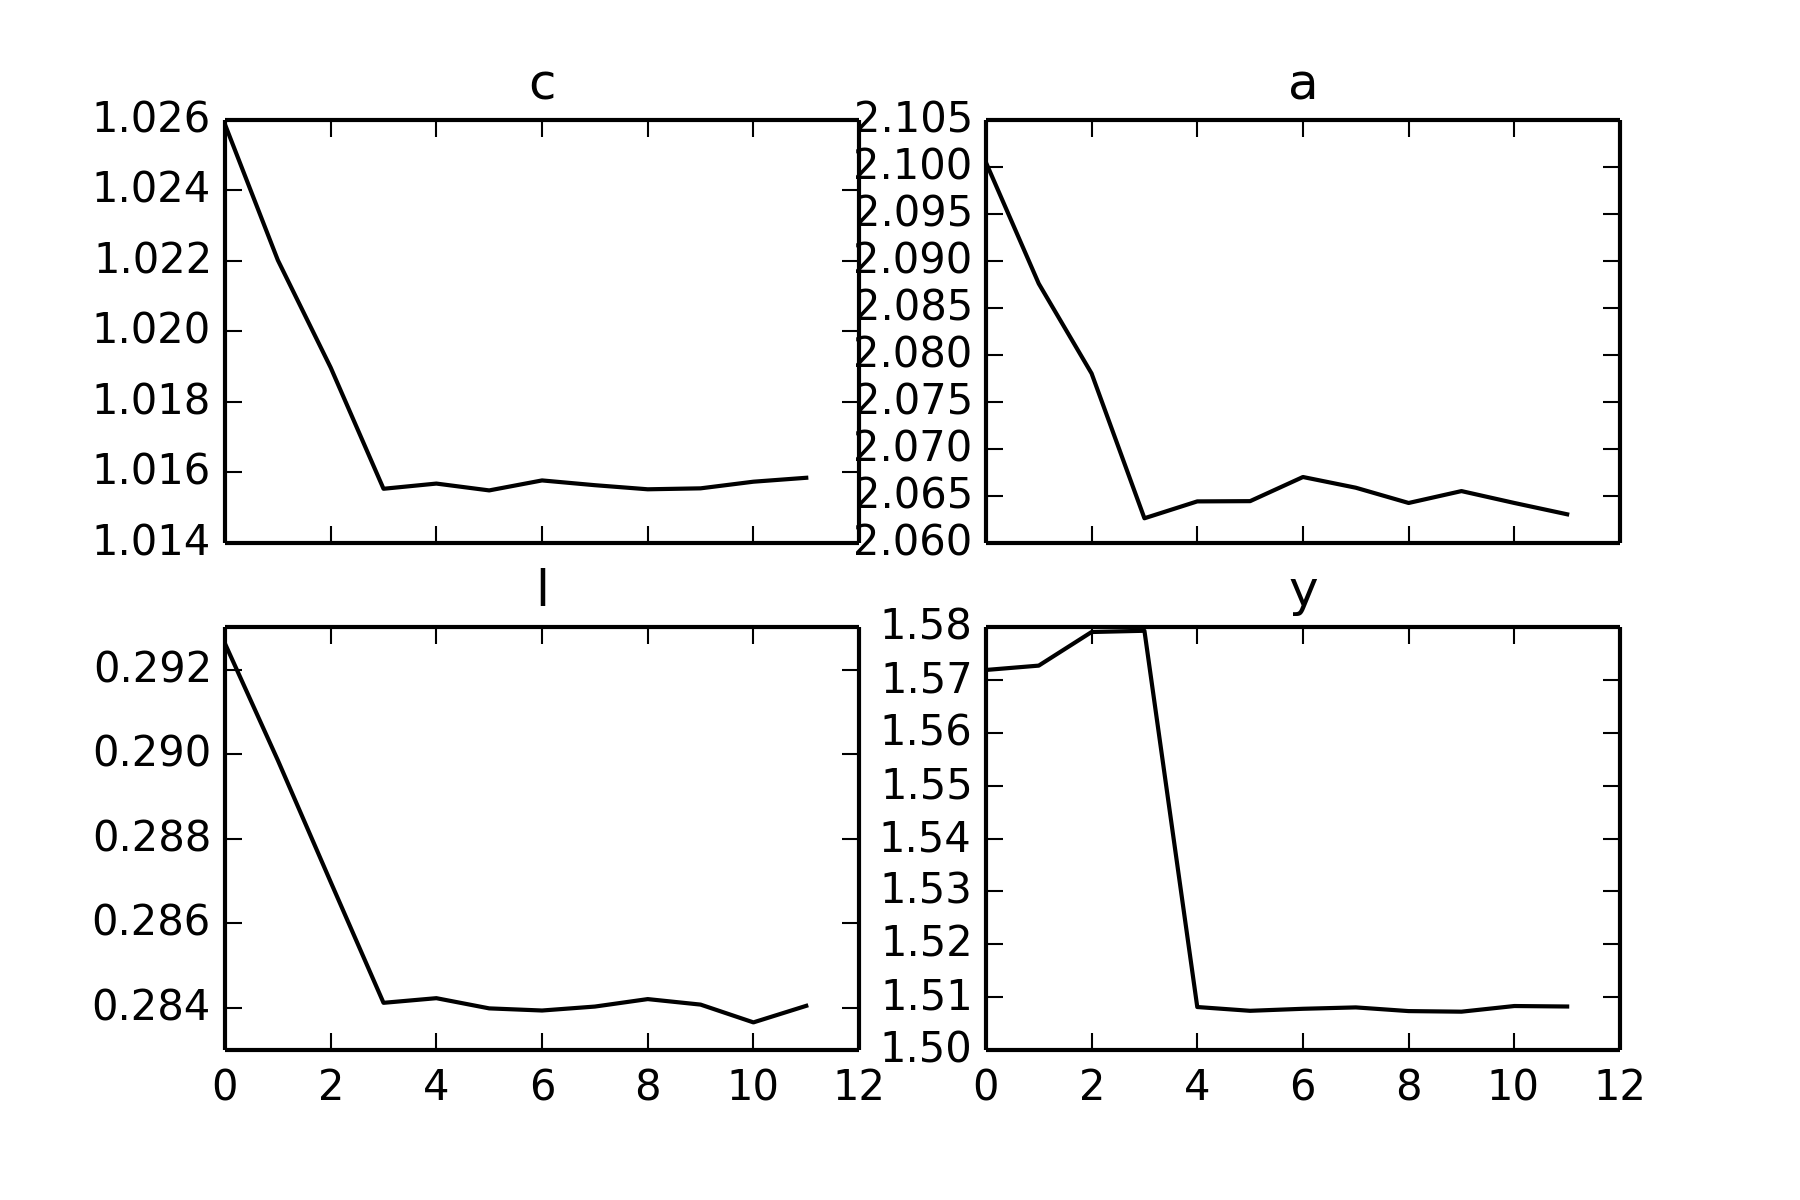
\includegraphics[width=\textwidth]{coeff_variation_bond_economy.png}
\caption{\tiny{Path for (cross-sectional) coefficient of variation after 5 periods of ``High'' TFP followed by no shocks}}
\label{fig:}
\end{figure}


 \end{frame}
 
 
\begin{frame}
 \frametitle{Procyclical payoffs}

\begin{figure}[htp]
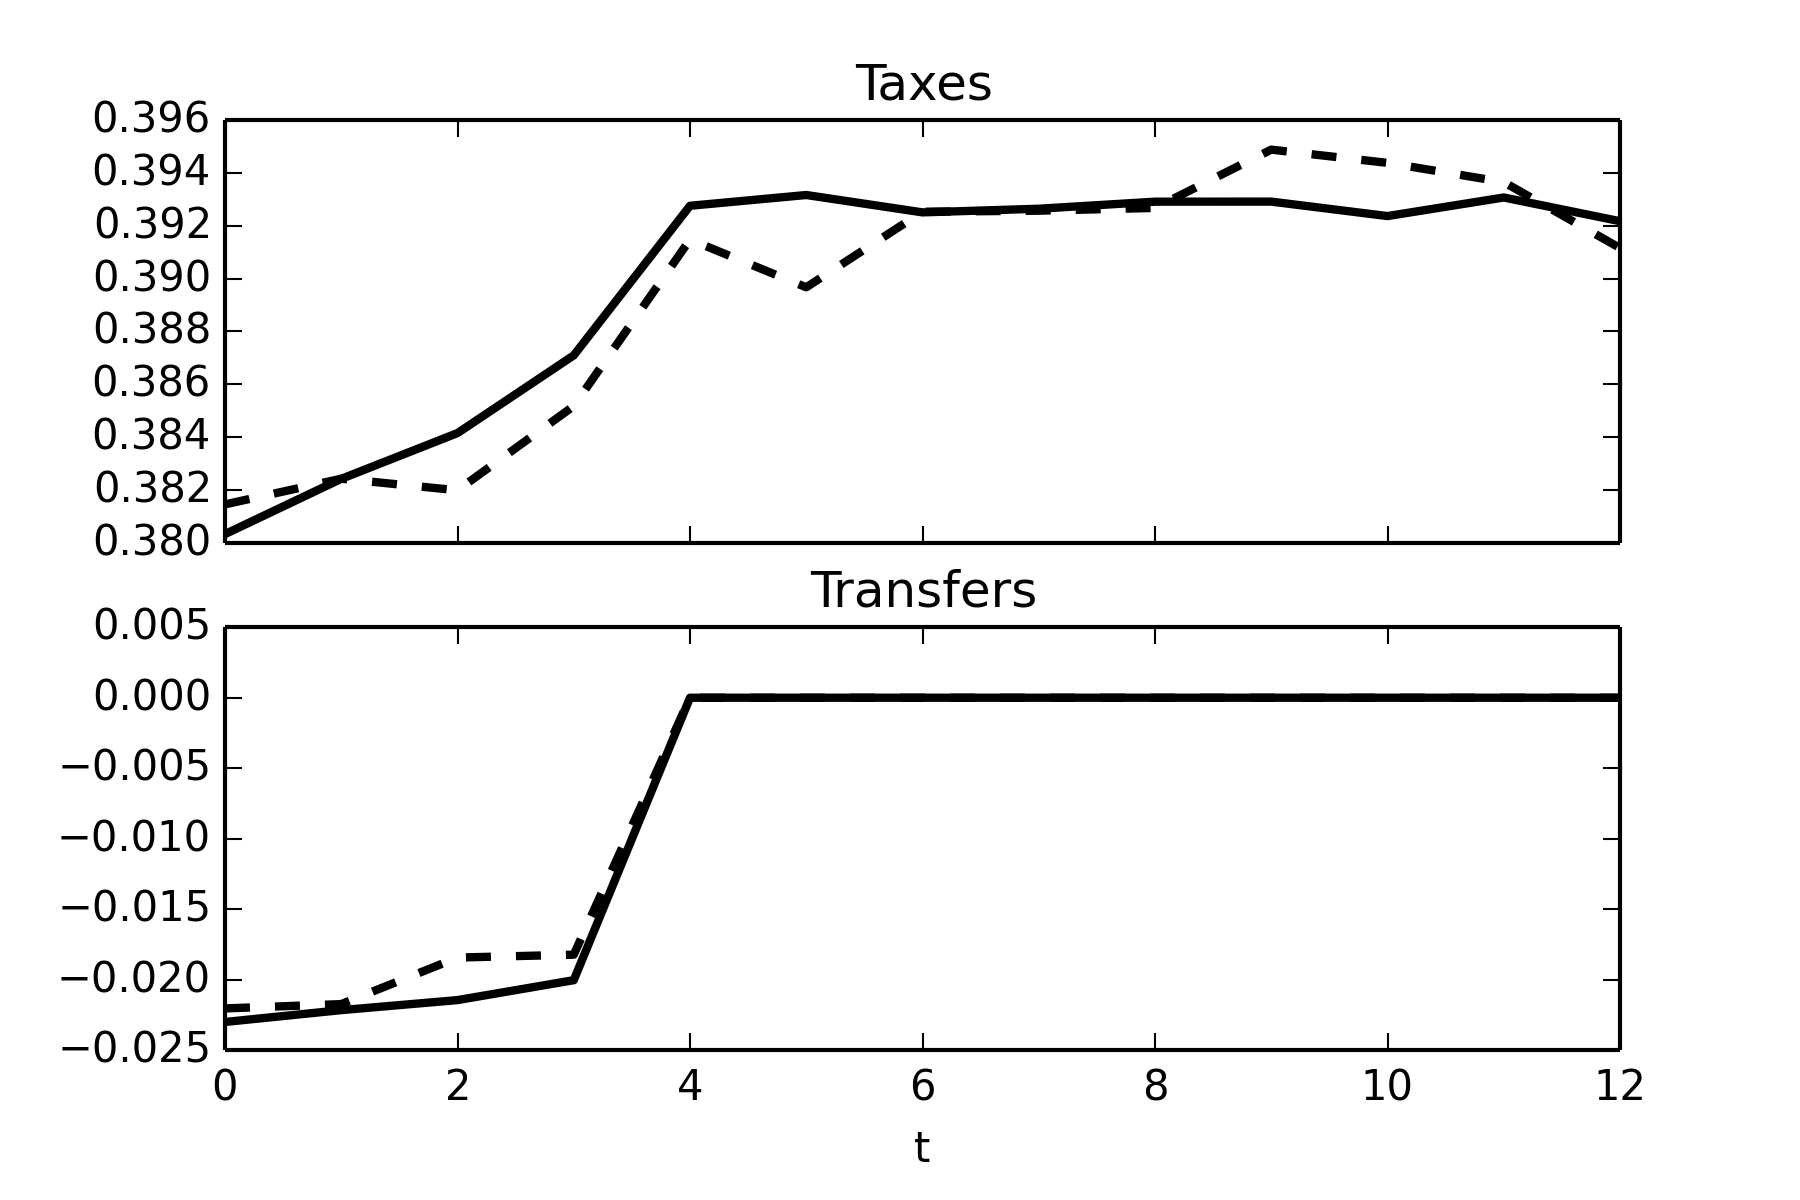
\includegraphics[width=\textwidth]{policy_irf_high_plot_data_procyclic_payoffs.png}
\caption{\tiny{This plots a ``impulse response'' (5 period of high aggregate TFP followed by no aggregate shocks) for taxes, transfers. The dotted (bold) line is the economy with (without) idiosyncratic risk}}
\label{fig:}
\end{figure}
 \end{frame}

 
 
 
 
 
\begin{frame}
 \frametitle{Changes in inequality: Procyclical payoffs}

\begin{figure}[htp]
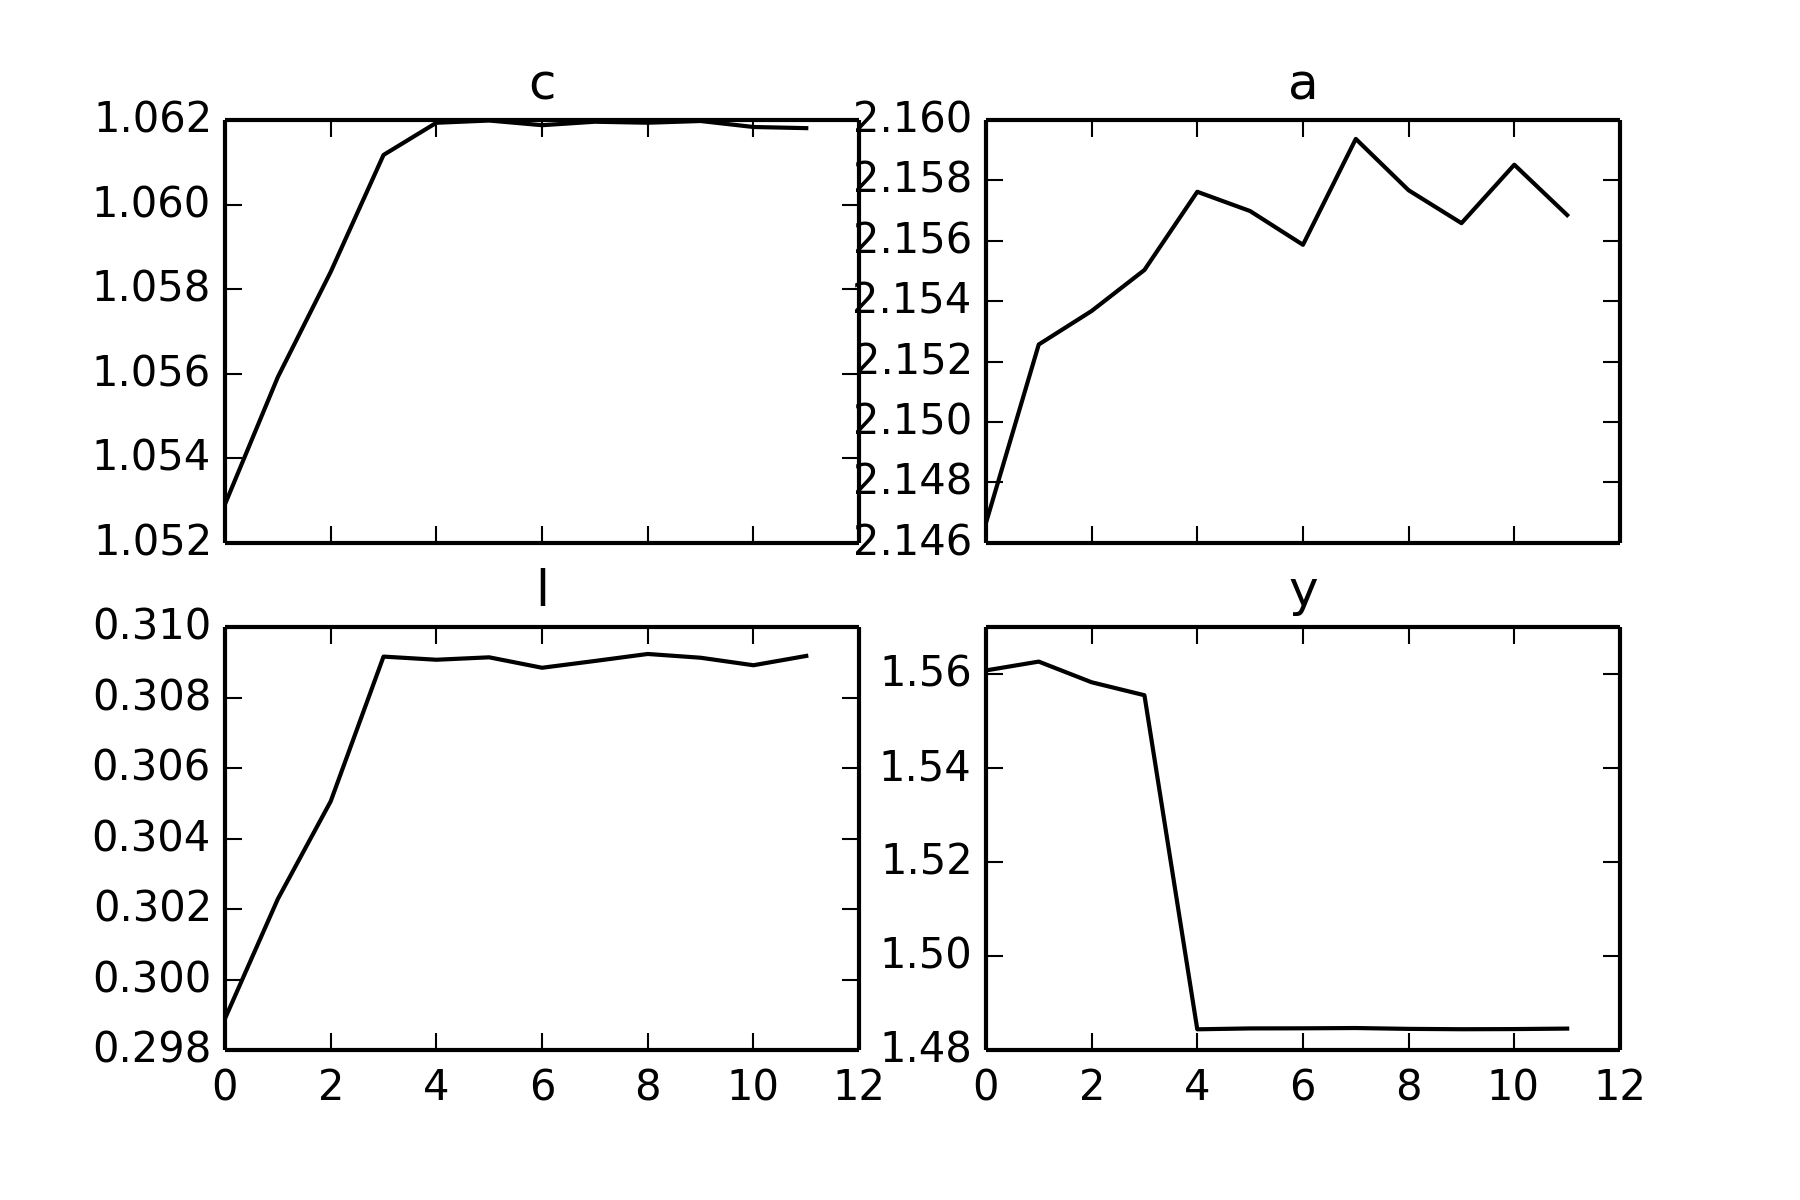
\includegraphics[width=\textwidth]{coeff_variation_procyclic_payoffs.png}
\caption{\tiny{Path for (cross-sectional) coefficient of variation after 5 periods of ``High'' TFP followed by no shocks}}
\label{fig:}
\end{figure}
 \end{frame}

 
 
 
 
 
 \begin{frame}
  \frametitle{Conclusions/Next Steps}
 
 
 \begin{itemize}
  \item Size of the debt alone does not matter
\item Optimal tax and transfer scheme balance
\begin{enumerate}
 \item welfare losses from fluctuating taxes
 \item welfare losses from fluctuating transfers
\end{enumerate}
\item Limits to fiscal hedging are key for dynamics of taxes and transfers

 \end{itemize}

 
 \textbf{Next Step:}
 \begin{itemize}
 \item Calibrate a richer model for idiosyncratic risk that allows for higher moments to vary systematically over business cycle
 \item More richer taxation scheme
 \end{itemize}
 
 
  

 \end{frame}
 

\begin{frame}

\frametitle{Ramsey problem: Recursive formulation}
\label{extra-slides}
Split  into two parts

\begin{enumerate}
\vspace{3mm}
\item $\mathbf{t\geq1}$: Ex-ante continuation problem with state variables $\{\Gamma_{t-1}(x_{i,t-1},m_{i,t-1},\theta_{i,t-1}),s_{t-1}\}$, where

\begin{itemize}
 \item Scaled assets: $x_{i,t-1}=u_{c,i,t-1}b_{i,t}$
 \item Scaled ``market weights'': $m_{i,t-1}\propto \frac{1}{u_{c,i,t-1}}$
\end{itemize}

% 
% \[\bm{x}= \beta_{t-1}^{-1}\left( U_{c,t-1}^{2}\tilde{b}_{2,t-1},...,U_{c,t-1}^{I}\tilde{b}_{I,t-1}\right)\]
% \[ \bm{\rho }=\left( U_{c,t-1}^{2}/U_{c,t-1}^{1},...,U_{c,t-1}^{I}/U_{c,t-1}^{1}\right) \]
\vspace{3mm}
\item $\mathbf{t=0} $: Ex-post initial problem with state variables $(\Psi_0(b_{i,-1}),s_{0})$
\end{enumerate}

\end{frame}

\begin{frame}
 \frametitle{Bellman Equation for  $t\geq1$}
 \scriptsize

\begin{equation*}
V(\Gamma_{\_},s\_)=\max_{\substack{c_{i}(s),l_{i}(s),x_{i}(s),m_{i}(s)\\\tau(s),T(s),\alpha_1,\alpha_2(s)} }
\sum_{s}\Pr (s|s\_)\left[ 
\int \omega_iu(c_i(s),l_i(s))di  +\beta V(\Gamma(s),s)\right]
\end{equation*}%



where the maximization is subject to
\begin{subequations}
\begin{equation*}
\label{eq-imp}
\frac{x_{i,\_}u_{i,c}(s)P(s|s\_)}  {\beta\mathbb{E}^i_{s\_}u_{i,c}(s)P(s|s\_)} = u_{i,c}(s)[c_i(s)-T(s)]+u_{i,l}(s)l_{i}(s)+x_i(s)
\end{equation*}



\begin{equation*}
\label{eq-Bond_1}
\alpha^1 =m_{i,\_}\mathbb{E}^i_{s\_}u_{i,c}(s)
\end{equation*}

\begin{equation*}
\label{eq-Bond_2}
\alpha^2(s)=m_i(s)u_{i,c}(s)
\end{equation*}

\begin{equation*}
\label{eq-wages}
-u_{i,l}(s)=[(1-\tau(s)] u_{i,c}(s) \theta_i(s)
\end{equation*}


\begin{equation*}
\label{eq-norm-m}
\int m_i(s) di=1
\end{equation*}

\begin{equation*}
\label{eq-resources}
\int l_i(s) \theta_i(s) di = \int c_i(s) di+g(s)
\end{equation*}
\end{subequations}

\end{frame}

\begin{frame}
\frametitle{Bellman equation for $t=0$}

 \begin{equation*}
V_0\left(\Psi_0(b_{i,-1}), s_0\right) = \max_{\substack{c_{i,0},l_{i,0},x_{i,0},m_{i,0}\\ \tau_0,T_0}} {\int \omega_i U^i(s_0) + \beta V\left(\Gamma_0, s_0\right)}
\end{equation*}
where the maximization is subject to
\begin{subequations}
%\textcolor{red}{XXXXX Should  a similar change to the one David recommended be executed here?}
\begin{equation*}
\label{eq-imp}
b_{i,-1}u_{i,c,0} = u_{i,c,0}[c_{i,0}-T_0]+u_{i,l,0}l_{i,0}+x_{i,0}
\end{equation*}



\begin{equation*}
\label{eq-wages}
-u_{i,l,0}=(1-\tau_0) u_{i,c,0} \theta_{i,0}
\end{equation*}


\begin{equation*}
\label{eq-norm-m}
\int m_{i,0} di=1
\end{equation*}

\begin{equation*}
\label{eq-resources}
\int l_{i,0} \theta_{i,0} di = \int c_{i,0} di+g_0
\end{equation*}
\end{subequations}

\hyperlink{ramsey-problem}{\beamerbutton{back}}
\end{frame}

 \end{document}